\chapter{Progettazione}

\section{Concettualizzazione}
Dopo aver raccolto ed analizzato i requisiti, è necessario individuare gli oggetti del dominio, codificandoli opportunamente in un formalismo logico.

\subsection{Incroci}

\begin{figure}[htb]
	\centering
	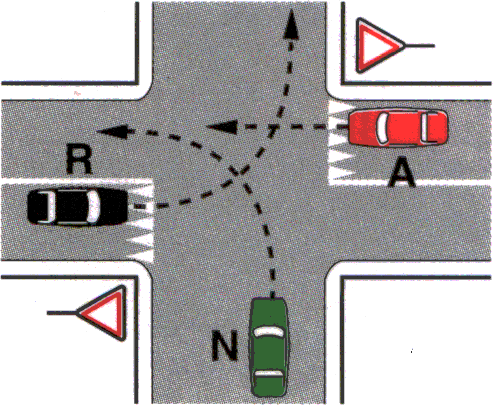
\includegraphics[width=.5\textwidth]{images/example}
	\caption{Esempio di incrocio}
	\label{fig:inc}
\end{figure}


Osservando l'immagine, si può procedere all'estrazione delle informazioni necessarie per costruire il sistema.

\subsubsection{Caso generale}

I veicoli sono caratterizzati dal loro colore, o dalla loro tipologia o una qualsiasi informazione utile per differenziarli. Inoltre si vuole conoscere da dove vengono e dove sono diretti, in particolare se hanno svoltato o hanno proseguito dritto. Occorre rappresentare anche la direzione e i bracci dell'incrocio.

Per identificare questo tipo di informazioni, una costruzione sensata potrebbe essere:
\begin{verbatim}
proviene(veicolo(nero), braccio(ovest)).
transita(veicolo(nero), sinistra, braccio(nord)).
\end{verbatim}

La struttura \texttt{proviene/2} ci indica quale veicolo va in un determinato braccio. Il predicato \texttt{veicolo/1} ha come operando un atomo che descrive in modo chiaro una caratteristica della macchina. Si potrebbe anche usare la lettera che accompagna l'auto nell'immagine, così da ottenere \texttt{veicolo(r)} (non maiuscola, altrimenti verrebbe scambiata per una variabile). Il braccio si affida alle \textbf{direzioni} della rosa dei venti, in questo caso \texttt{ovest}. Le direzioni possibili sono otto, come in figura:

\begin{figure}[htb]
	\centering
	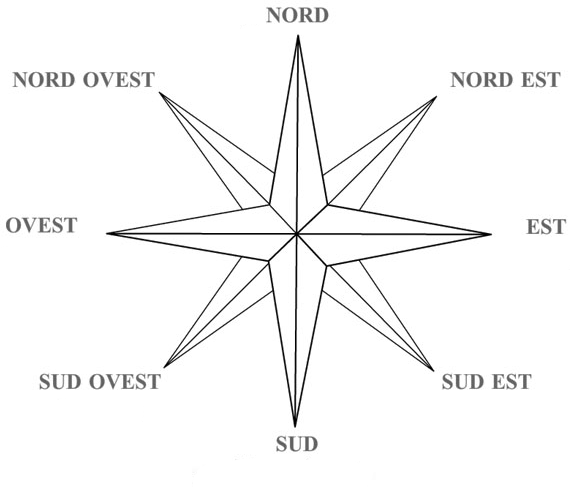
\includegraphics[width=.5\textwidth]{images/rose}
	\caption{Rosa dei venti}
\end{figure}

Nella figura \ref{fig:inc} si nota la presenza di due segnali stradali. In questo caso, la costruzione sarebbe:
\begin{verbatim}
si_trova(segnale(dare_precedenza), braccio(est)).
si_trova(segnale(dare_precedenza), braccio(ovest)).
\end{verbatim}

La relazione \texttt{si\_trova/2} indica quale segnale si trova in un determinato braccio, analogamente a \texttt{proviene/2}. I segnali presi in considerazione sono due, il \fbox{Dare precedenza} e lo \fbox{STOP}:

\begin{center}
	\begin{tabularx}{\textwidth} {lX}
		\adjustbox{valign=t}{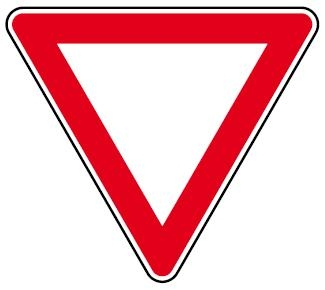
\includegraphics[width=1.5cm]{images/dareprec}} & \textbf{Dare precedenza}: prescrive di dare la precedenza ai veicoli circolanti sulla strada che si incrocia o su cui ci si immette (sia da destra che da sinistra). \\
		
		\adjustbox{valign=t}{
\includegraphics[width=1.5cm]{images/stop}} & \textbf{STOP}: obbliga a fermarsi in corrispondenza della striscia trasversale, anche se non c'è nessuno, e dare la precedenza ai veicoli provenienti sia da destra che da sinistra. 
	\end{tabularx}
\end{center}

Gli altri segnali che garantiscono un diritto di precedenza vengono tralasciati perché il focus è dato all'aspetto passivo del comportamento dei veicoli, non a quello attivo. Nel caso in cui l'incrocio non dovesse presentare segnali, \texttt{si\_trova/2} non verrebbe usato.


Tutti questi fatti costituiscono un unico oggetto, l'incrocio stesso, che viene memorizzato su una \emph{base di conoscenza} per poter essere sfruttato in seguito. L'incrocio quindi è descritto da un ID, ad esempio il numero dell'incrocio, e la lista dei termini descritti sopra. In particolare, l'incrocio in figura \ref{fig:inc} diventa:
\begin{verbatimtab}
incrocio(fig633, [
	proviene(veicolo(nero), braccio(ovest)),
	proviene(veicolo(rosso), braccio(est)),
	proviene(veicolo(verde), braccio(sud)),
	transita(veicolo(nero), sinistra, braccio(nord)),
	transita(veicolo(rosso), dritto, braccio(ovest)),
	transita(veicolo(verde), sinistra, braccio(ovest)),
	si_trova(segnale(dare_precedenza), braccio(est)),
	si_trova(segnale(dare_precedenza), braccio(ovest))
]).
\end{verbatimtab}

\subsubsection{Incroci con priorità}

Esistono incroci in cui vengono coinvolti veicoli con priorità differenti, dovute a situazioni di emergenza o a condizioni particolari del veicolo, che quindi ignorano le normali situazioni di precedenza, se non specificato altrimenti.

I veicoli che si ritrovano in situazioni di emergenza sono le ambulanze, i veicoli delle forze dell'ordine e i camion dei vigili del fuoco, se accompagnati dalla scritta ``situazione di soccorso", ``in emergenza", ``sirena in funzione" o simili. I tram ed altri veicoli su rotaia hanno la precedenza su quelli normali, tranne che sui veicoli in emergenza.


\begin{figure}[htbp!]
	\centering
	\begin{subfigure}{.3\textwidth}
		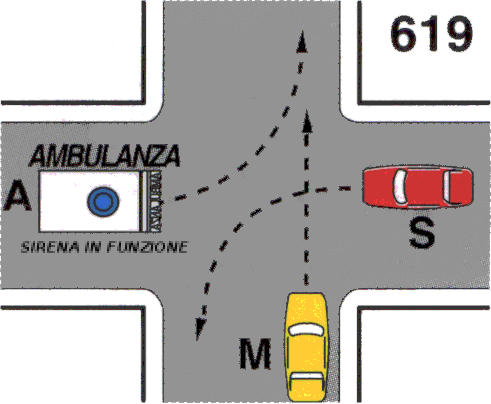
\includegraphics[width=\textwidth]{./images/ambulance}
		\caption{Ambulanza}
		\label{fig:amb}
	\end{subfigure}
	\begin{subfigure}{.3\textwidth}
		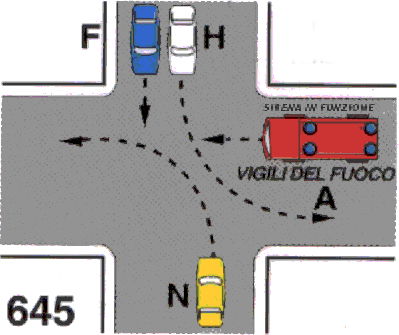
\includegraphics[width=\textwidth]{./images/fire}
		\caption{Vigili del fuoco}
		\label{fig:fire}
	\end{subfigure}
	\begin{subfigure}{.3\textwidth}
		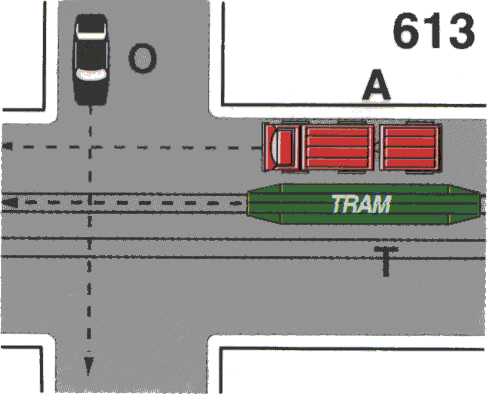
\includegraphics[width=\textwidth]{./images/tram}
		\caption{Tram}
		\label{fig:tram}
	\end{subfigure}
	\caption{Incroci con veicoli prioritari}
	\label{fig:prior}
\end{figure}

\subsubsection{Attesa circolare}
I veicoli coinvolti in un incrocio potrebbero trovarsi in una situazione di stallo, dove nessuno passa per primo sotto le normali condizioni di precedenza. Un veicolo, di solito quello che transita a sinistra, si porta al centro dell'incrocio, lascia passare gli altri secondo l'ordine di precedenza e passa per ultimo, risolvendo lo stallo:

\begin{figure}[htb]
	\centering
	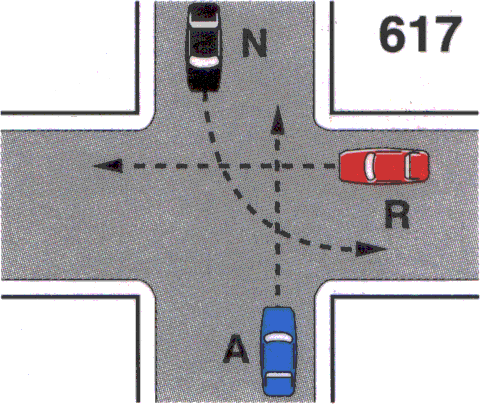
\includegraphics[width=.5\textwidth]{images/lock}
	\caption{Incrocio con stallo}
\end{figure}

\subsection{Precedenze}
Possono essere fatte varie tassonomie sulle precedenze, secondo diversi punti di vista. Qui ne vengono presentati quattro.
\subsubsection{Precedenza a destra}
Secondo il comma 2 del CdS disponibile in \ref{sec:prec}, un veicolo ha l'obbligo di dare la precedenza a chi gli viene da destra, salvo diversa segnalazione.

\subsubsection{Precedenza frontale}
Un veicolo non deve solo badare a dare la precedenza a destra quando si è fermi all'incrocio, ma anche quando nella sua manovra esso si ritrovi ad incrociare un veicolo alla sua destra. La precedenza cosiddetta ``frontale"" è un'estensione di quella a destra. Esistono due casi:
\begin{center}
	\begin{tabularx}{\textwidth} {lX}
		\adjustbox{raise=-3.5cm}{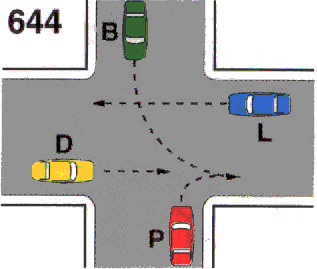
\includegraphics[width=.4\textwidth]{images/front}} & Il veicolo \textbf{B} deve dare precedenza frontale al veicolo \textbf{P}. Se due veicoli vanno nello stesso braccio, uno svoltando a destra e l'altro a sinistra, quello che va a sinistra deve dare la precedenza a quello che va a destra. \\
		
		\adjustbox{raise=-3.5cm}{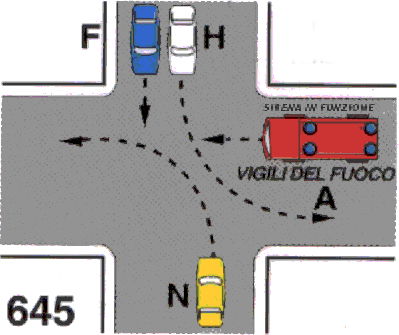
\includegraphics[width=.4\textwidth]{images/fire}} & Il veicolo \textbf{N} deve dare precedenza frontale al veicolo \textbf{F}. Se un veicolo, svoltando a sinistra, incrocia un veicolo che, proseguendo dritto, si dirige nel braccio di provenienza del primo, esso deve dare la precedenza al veicolo che va dritto.
	\end{tabularx}
\end{center}


\subsubsection{Precedenza con segnale}
I segnali, come già detto sopra, sono il \fbox{Dare precedenza} e lo \fbox{STOP}, che costringono il veicolo ad avere un comportamento passivo nei confronti degli altri veicoli e a dare obbligatoriamente la precedenza.

\subsubsection{Precedenza con priorità}
I veicoli che hanno la sirena accesa, di fatto in situazione di emergenza (ambulanze, autopompe ecc.), hanno la precedenza su tutti. I tram e i veicoli su rotaia la danno solamente ai veicoli in stato di soccorso e ce l'hanno nei confronti degli altri veicoli. Nel caso estremo due veicoli in emergenza si trovino ad un'intersezione, valgono le normali condizioni di precedenza, visto che il CdS non descrive questa situazione particolare, definendo magari eccezioni o deroghe. Sta di fatto che questo caso è difficile da risolvere anche nella realtà.

\subsection{Circolazione}
È importante capire qual è l'ordine di circolazione dei veicoli. Per prima cosa bisogna analizzare lo stato dell'incrocio, se è a scorrimento normale o sono presenti degli stalli, o un caso misto. Nel primo caso vengono identificate tre fasi:
\begin{enumerate}
	\item Il gruppo di veicoli che passa prima, ossia quei veicoli che non vengono preceduti da nessuno e a loro volta precedono qualcuno.
	\item Il gruppo di veicoli che passa dopo, formato dai veicoli che non sono nè primi nè ultimi e che devono essere smistati nel giusto ordine.
	\item Il gruppo di veicoli che passa per ultimo, dove i veicoli non precedono nessuno e sono preceduti da almeno un veicoli.
\end{enumerate}

Ci possono essere fasi in cui più veicoli passano contemporaneamente, in particolare ci possono essere ``più primi" e ``più ultimi". Anche nella seconda fase ci possono essere veicoli simultanei, o una successione, o entrambi i casi. Nel caso della sequela di veicoli nella seconda fase. i veicoli vengono ordinati secondo le precedenze degli uni sugli altri.
\\\\
In presenza di uno stallo vengono lo stesso identificate tre fasi, se pur diverse:
\begin{enumerate}
	\item Prima di uno stallo per verificare se ci sono veicoli, non coinvolti nello stallo, che passano prima.
	\item Durante lo stallo, dove davvero si tenta di sbloccare i veicoli.
	\item Infine, dopo lo stallo, che è come la prima fase sostanzialmente, ma viene controllato se ci siano veicoli che passano dopo che lo stallo è stato risolto.
\end{enumerate}
